\documentclass[landscape]{sintefposter}

\usepackage{hyperref,multicol,wrapfig}
\usepackage{tcolorbox}
\usepackage{fancyvrb}

\title{SpliPy$^{1.3}$ - Spline modelling in Python}

\author{Eivind Fonn, Kjetil Andre Johannessen }

\institute{SINTEF Digital, Dept. of Mathematics and Cybernetics, Trondheim, Norway}

\email{Eivind.Fonn@sintef.no, Kjetil.Johannessen@sintef.no}

\conference{SIN\TeX project}

\graphicspath{{.}{Figures/}}

\begin{document}
\leftlogo{splipylogo}
\maketitle

\begin{multicols}{3}
\section{Introduction}
\begin{tcolorbox}[colback=sintefblue!10!white,colframe=sintefblue,title=Abstract]
  Splipy is a pure python library for the creation, evaluation and manipulation of B-spline and NURBS geometries.
  It supports $n$-variate splines of any dimension, but emphasis is made on the use of curves, surfaces and volumes.
  The library is designed primarily for analysis use, and therefore allows fine-grained control over many aspects which is not possible to achieve with conventional CAD tools.
\end{tcolorbox}
\textbf{Keywords:} NURBS, B-splines, CAD, Interpolation, Approximation
\vspace{1cm}

\begin{tcolorbox}[colback=white,colframe=sintefblue,title=Installation]
  The package is distributed through the Python Package Index (PyPI) and can be installed by typing
  \begin{tcolorbox}[colback=sinteflightgrey]
  \begin{verbatim}
> pip install splipy \end{verbatim}
  \end{tcolorbox}
  into the commandline; or anaconda promt
\end{tcolorbox}

\section{B-splines}
Given a knot vector of nondecreasing knots $\Xi=[\xi_1, \xi_2, \xi_3, ... \xi_{n+p+1}]$ we define the set of $n$ basisis functions by
\begin{tcolorbox}[colback=sintefblue!10!white,colframe=sintefblue,title=The basis]
  \begin{equation}
    \label{eq:bspline}
    N_{i,p}(\xi) = \frac{\xi - \xi_i}{\xi_{i+p}-\xi_i}N_{i,p-1}(\xi) + \frac{\xi_{i+p+1}-\xi}{\xi_{i+p+1}-\xi_{i+1}}N_{i+1,p-1}(\xi),
  \end{equation}
  and,
  \begin{equation}
    \label{eq:bspline-start}
    N_{i,0}(\xi) = \left\{
    \begin{array}{ll}
      1  &  $if $ \ \ \xi \in [\xi_i, \xi_{i+1}) \\
      0  &  $else$
    \end{array}
    \right.
  \end{equation}
\end{tcolorbox}

By creating a tensor product of two or three univariate splines weighted by their controlpoints $\mathbf{B}_{i,j}$, we are able to create surface and solid representations, i.e.
\begin{equation}
  \mathbf{F}(\xi,\eta) = \sum_{i=1}^n \sum_{j=1}^n \mathbf{B}_{i,j} N_{i,p}(\xi)N_{j,q}(\eta)
\end{equation}
for bivariate surfaces.

\begin{center}
  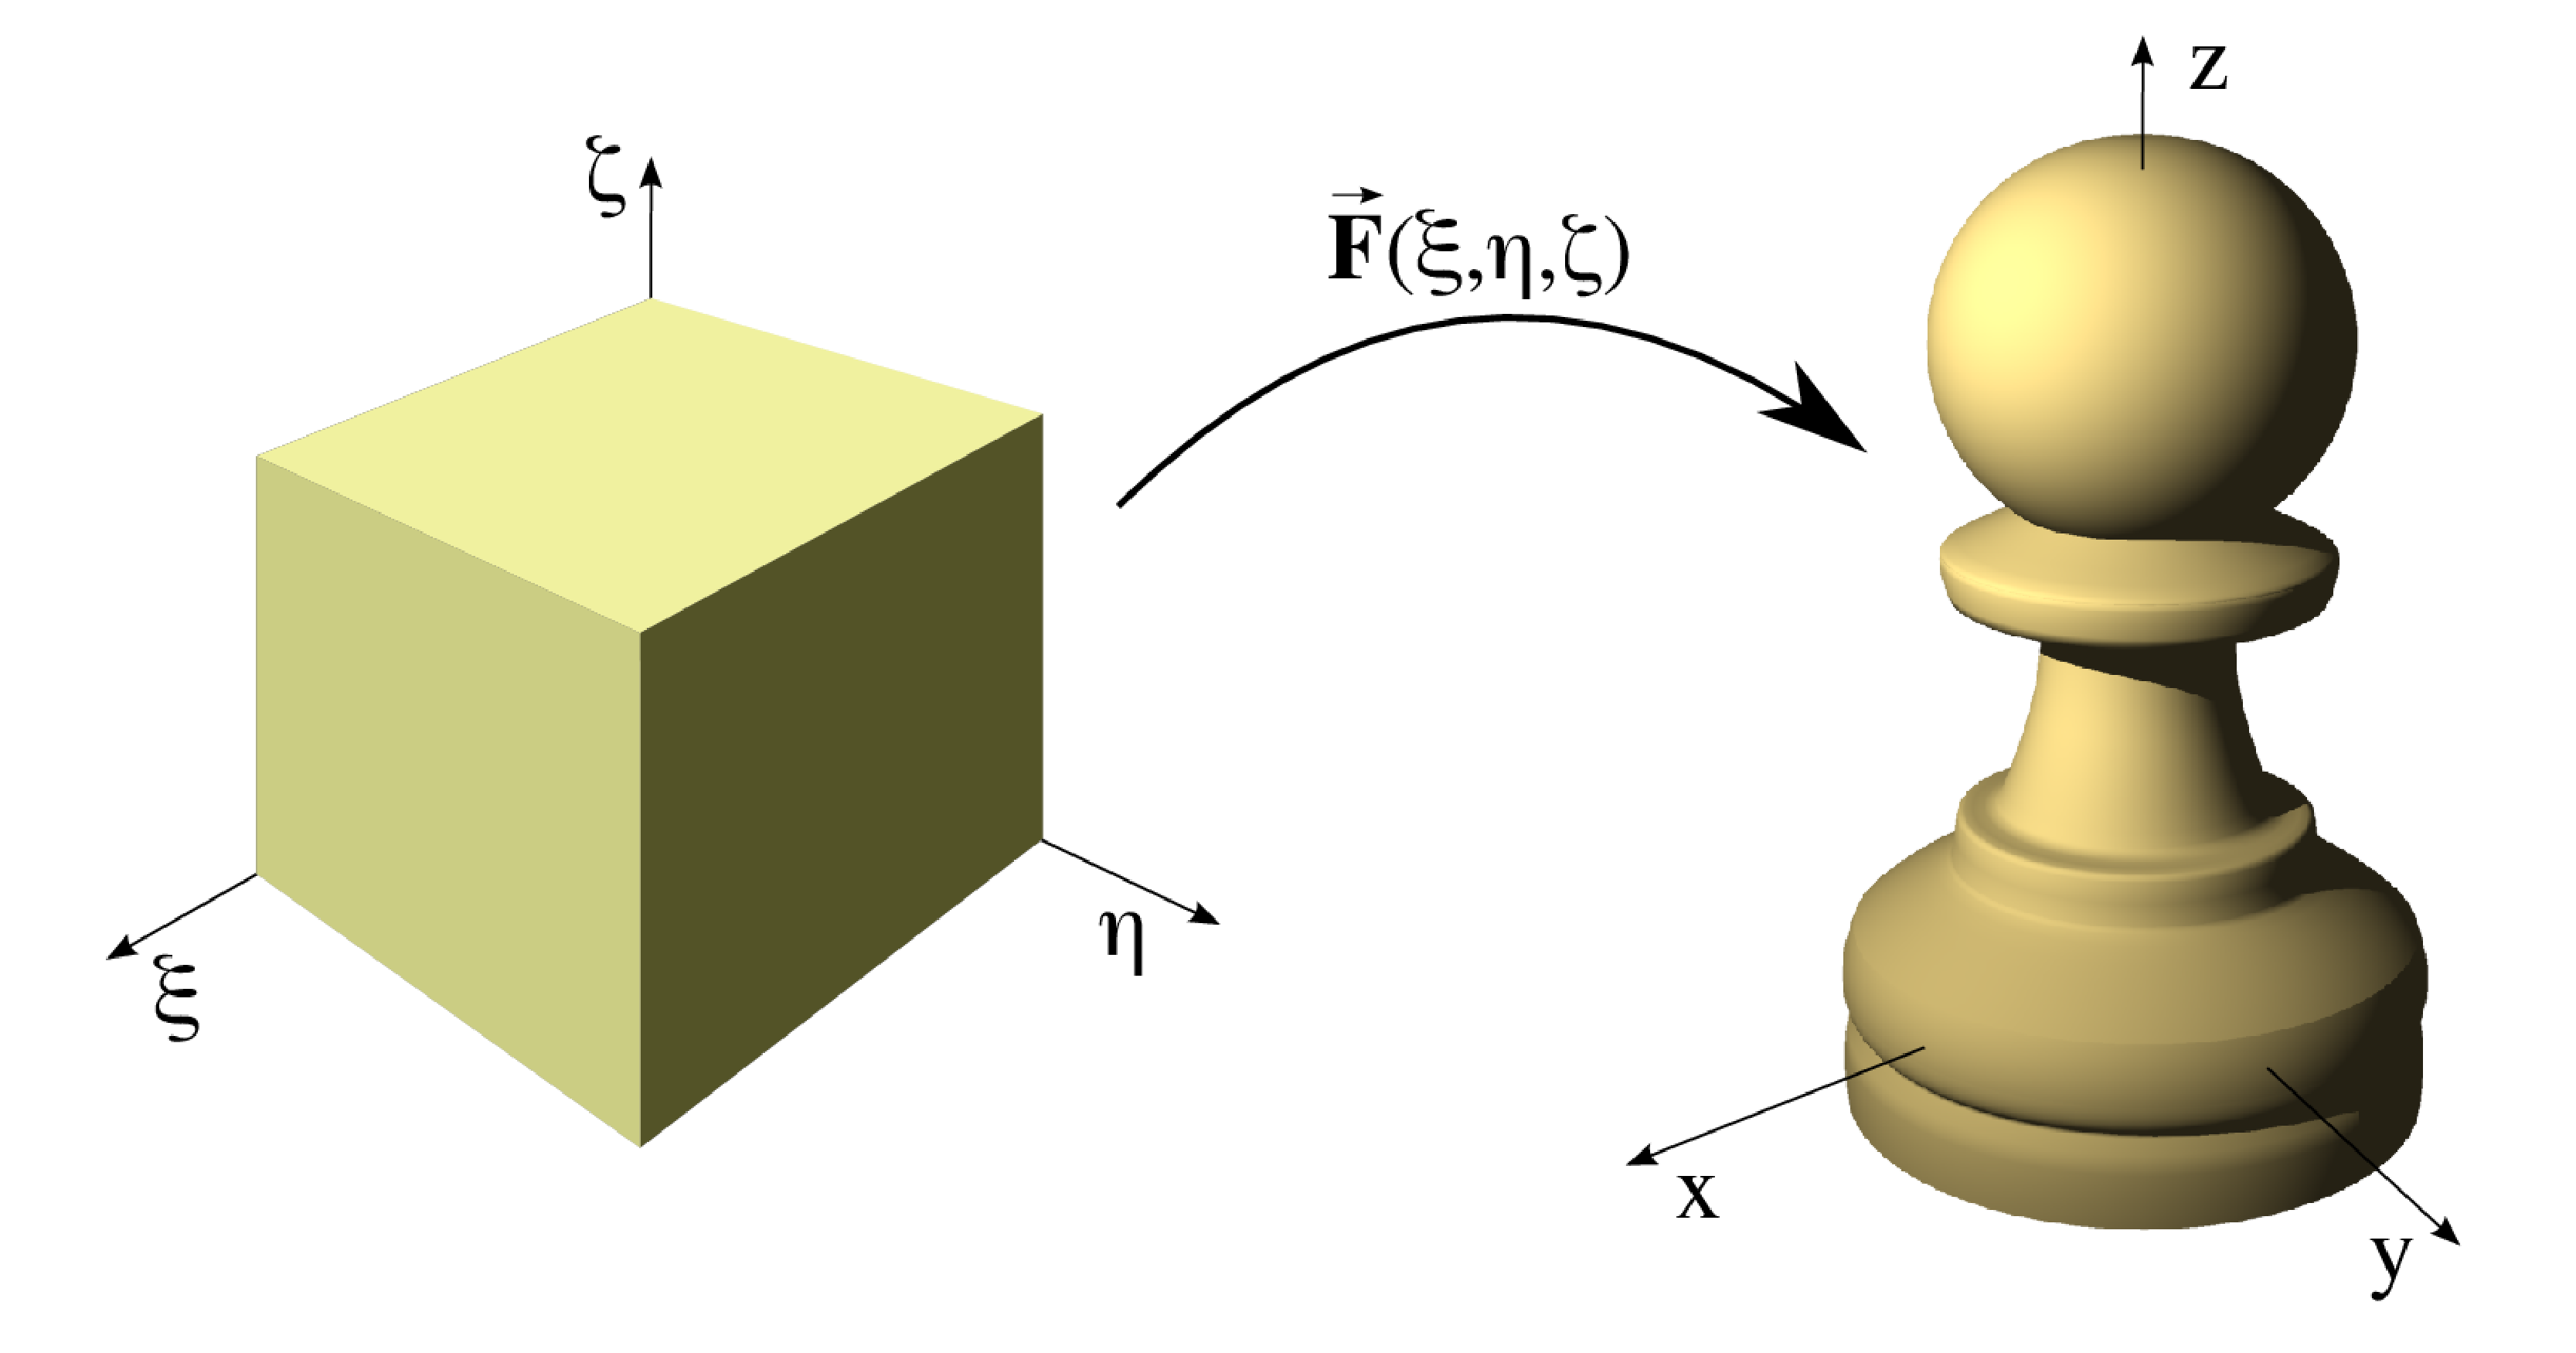
\includegraphics[width=16cm]{pawn-mapping}
  
\includegraphics[height=5cm]{MappingQR} \\
  \normalsize{Fig 1: A trivariate NURBS solid mapping}
\end{center}

\section{Structure}

The class follows a quite simple structure with a Curve, Surface and Volume class which all inherit from a parent SplineObject class. Corresponding to each of these primtitives, we collect a number of generative methods in so-called factory classes.

\begin{center}
  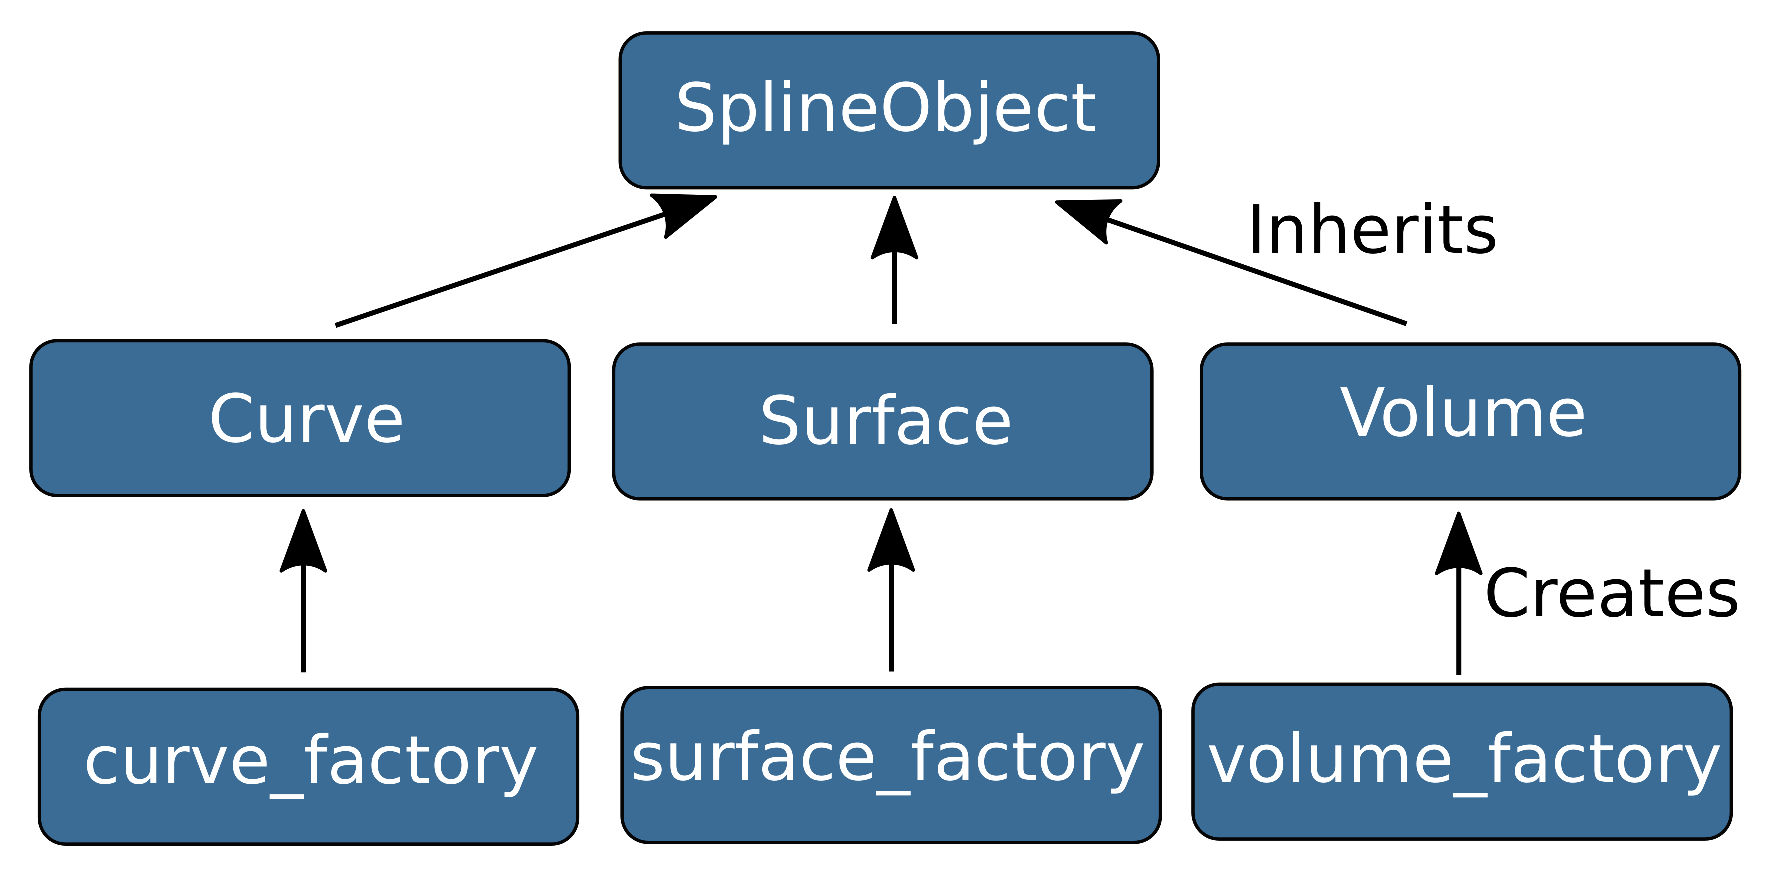
\includegraphics[width=0.7\linewidth]{classstructure} \\
  \normalsize{Fig 2: Primary classes and modules}
\end{center}

\section{Examples}

\begin{tcolorbox}[colback=white,colframe=sintefblue,title=Airfoil meshing]
  \begin{figure}[ht]
    \begin{center}
      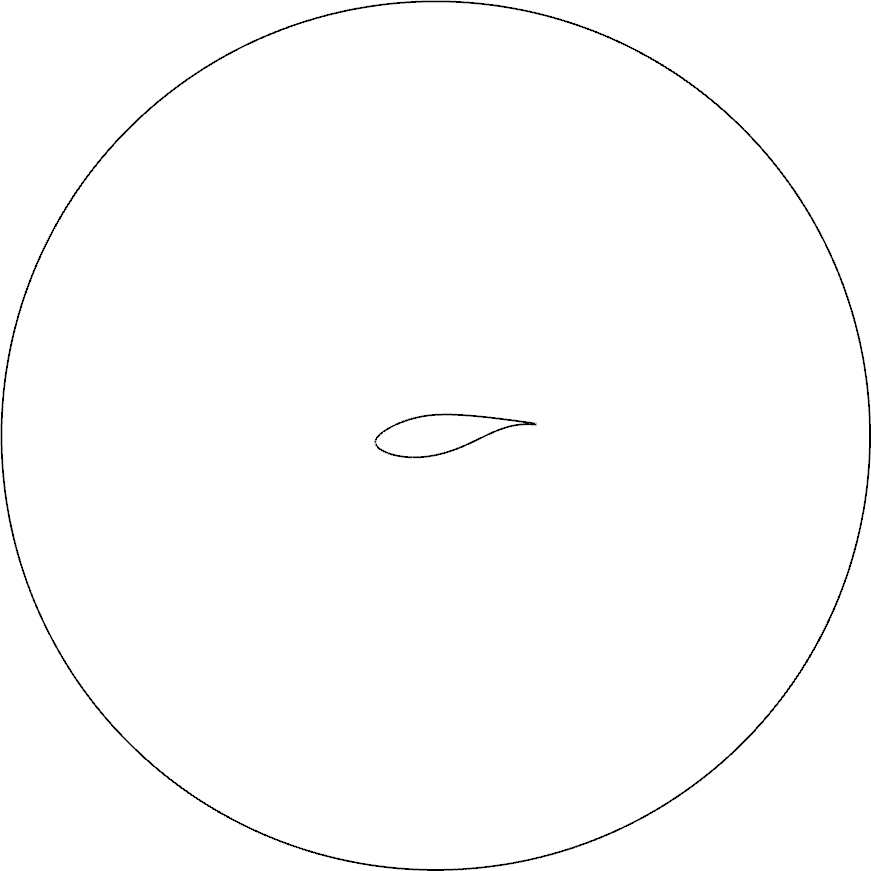
\includegraphics[width=0.24\textwidth]{Figures/tfi-1}
      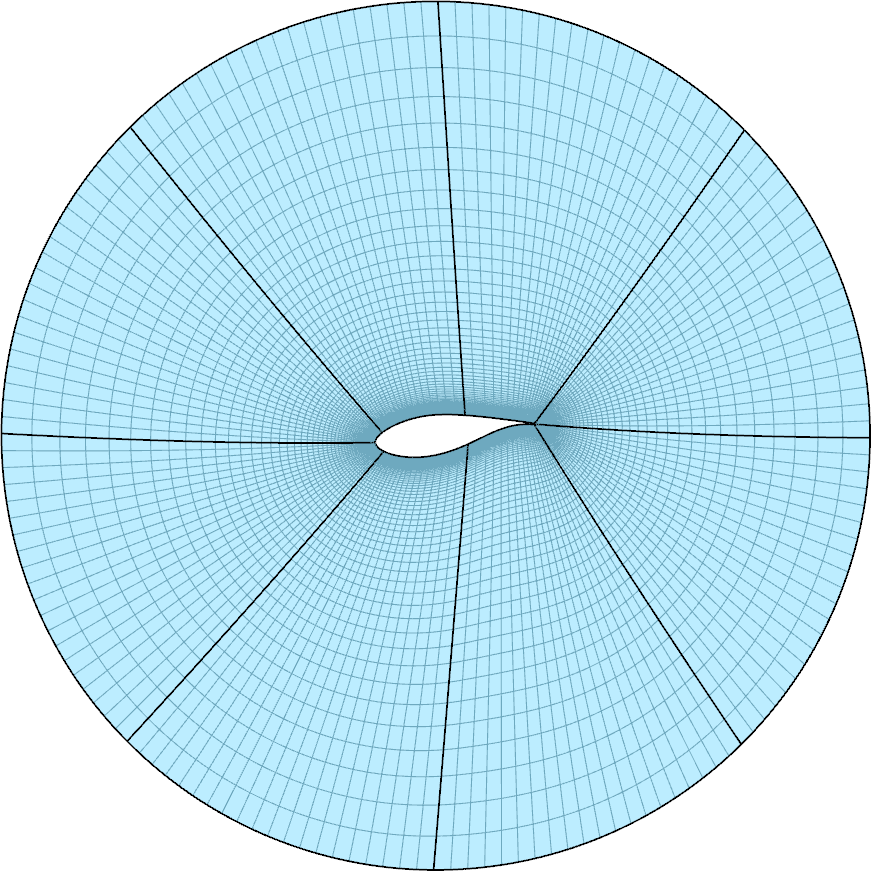
\includegraphics[width=0.24\textwidth]{Figures/tfi-2}
      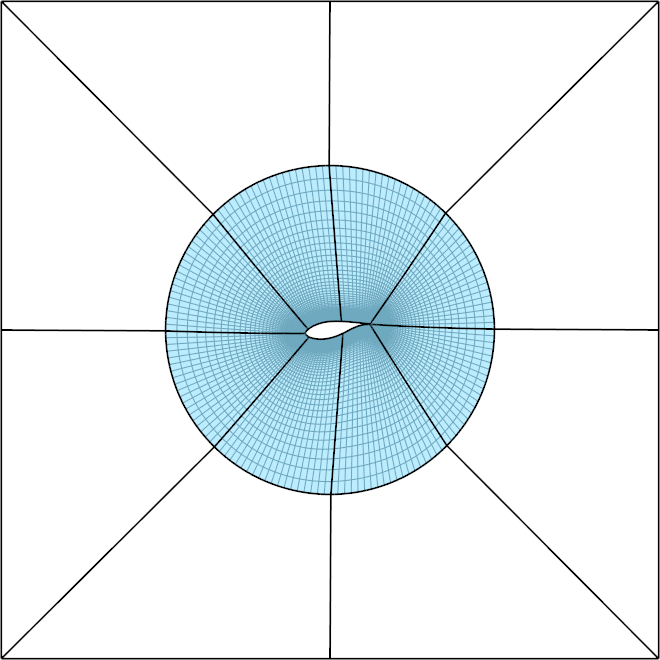
\includegraphics[width=0.24\textwidth]{Figures/tfi-3}
      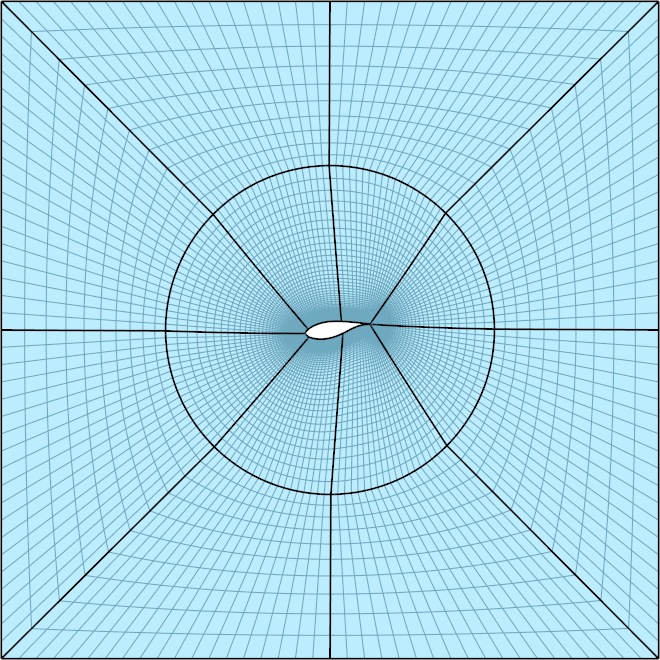
\includegraphics[width=0.24\textwidth]{Figures/tfi-4} \\
      \normalsize{
        Fig 3: Line-to-surface construction of ``O-mesh'' around an airfoil.
      }
    \end{center}
  \end{figure}
\end{tcolorbox}
\begin{tcolorbox}[colback=white,colframe=sintefblue,title=Wingtip meshing]
  \begin{figure}[ht]
    \begin{center}
      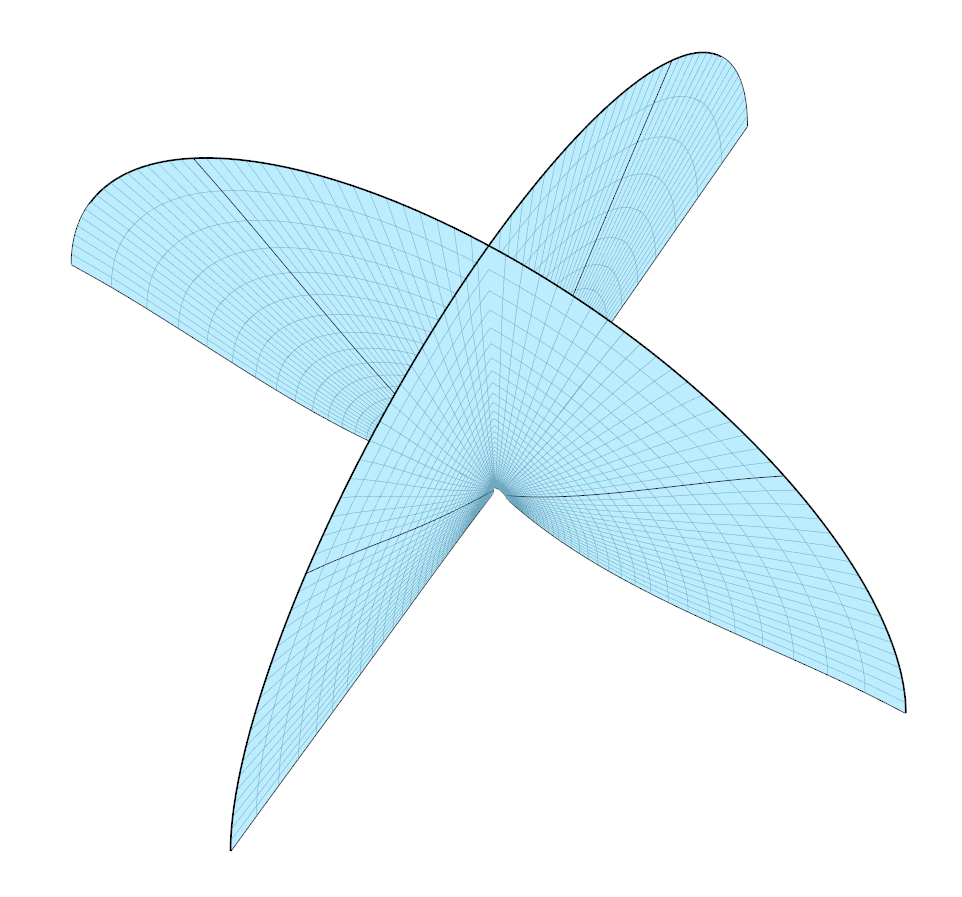
\includegraphics[width=0.24\textwidth]{Figures/wingtip-first}
      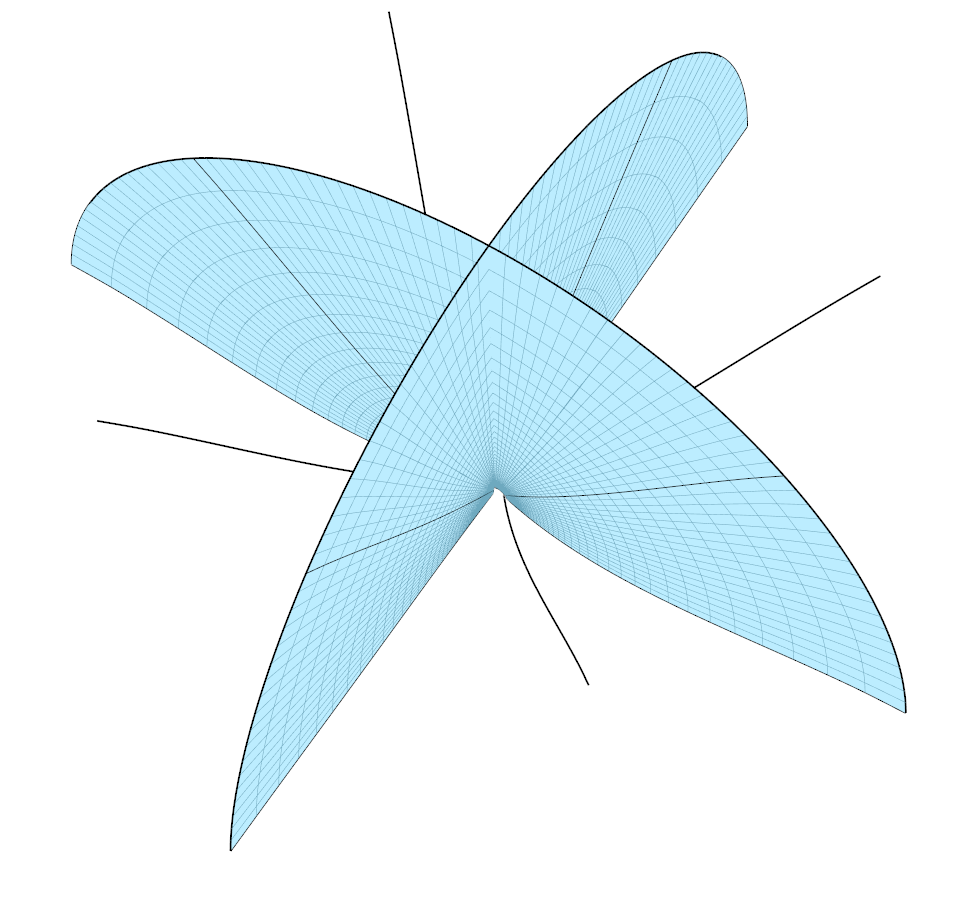
\includegraphics[width=0.24\textwidth]{Figures/wingtip-centers}
      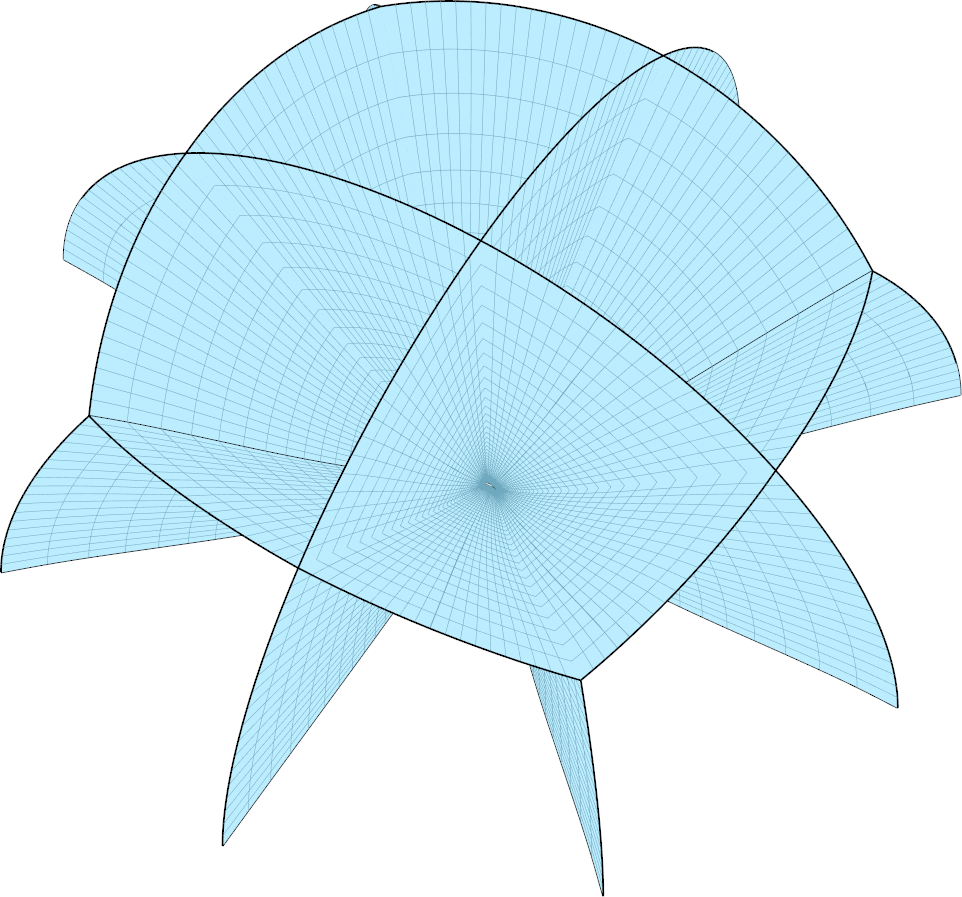
\includegraphics[width=0.24\textwidth]{Figures/wingtip-flower} \\
      \normalsize{
        Fig 4: Line-to-surface construction of ``flower mesh'' around a wingtip.
      }
    \end{center}
  \end{figure}
\end{tcolorbox}
\begin{tcolorbox}[colback=white,colframe=sintefblue,title=Windturbine blade]
  \begin{figure}[ht]
    \begin{center}
      \raisebox{1.3cm}{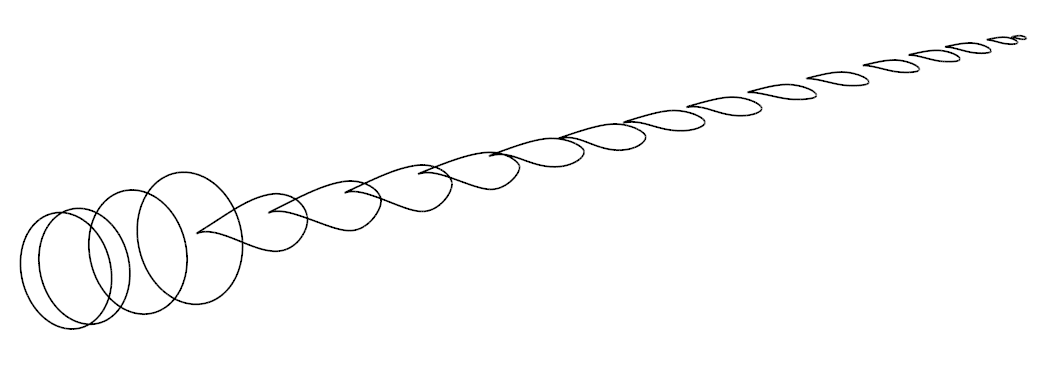
\includegraphics[width=0.32\textwidth]{Figures/cross-airfoils}}
      \raisebox{0.4cm}{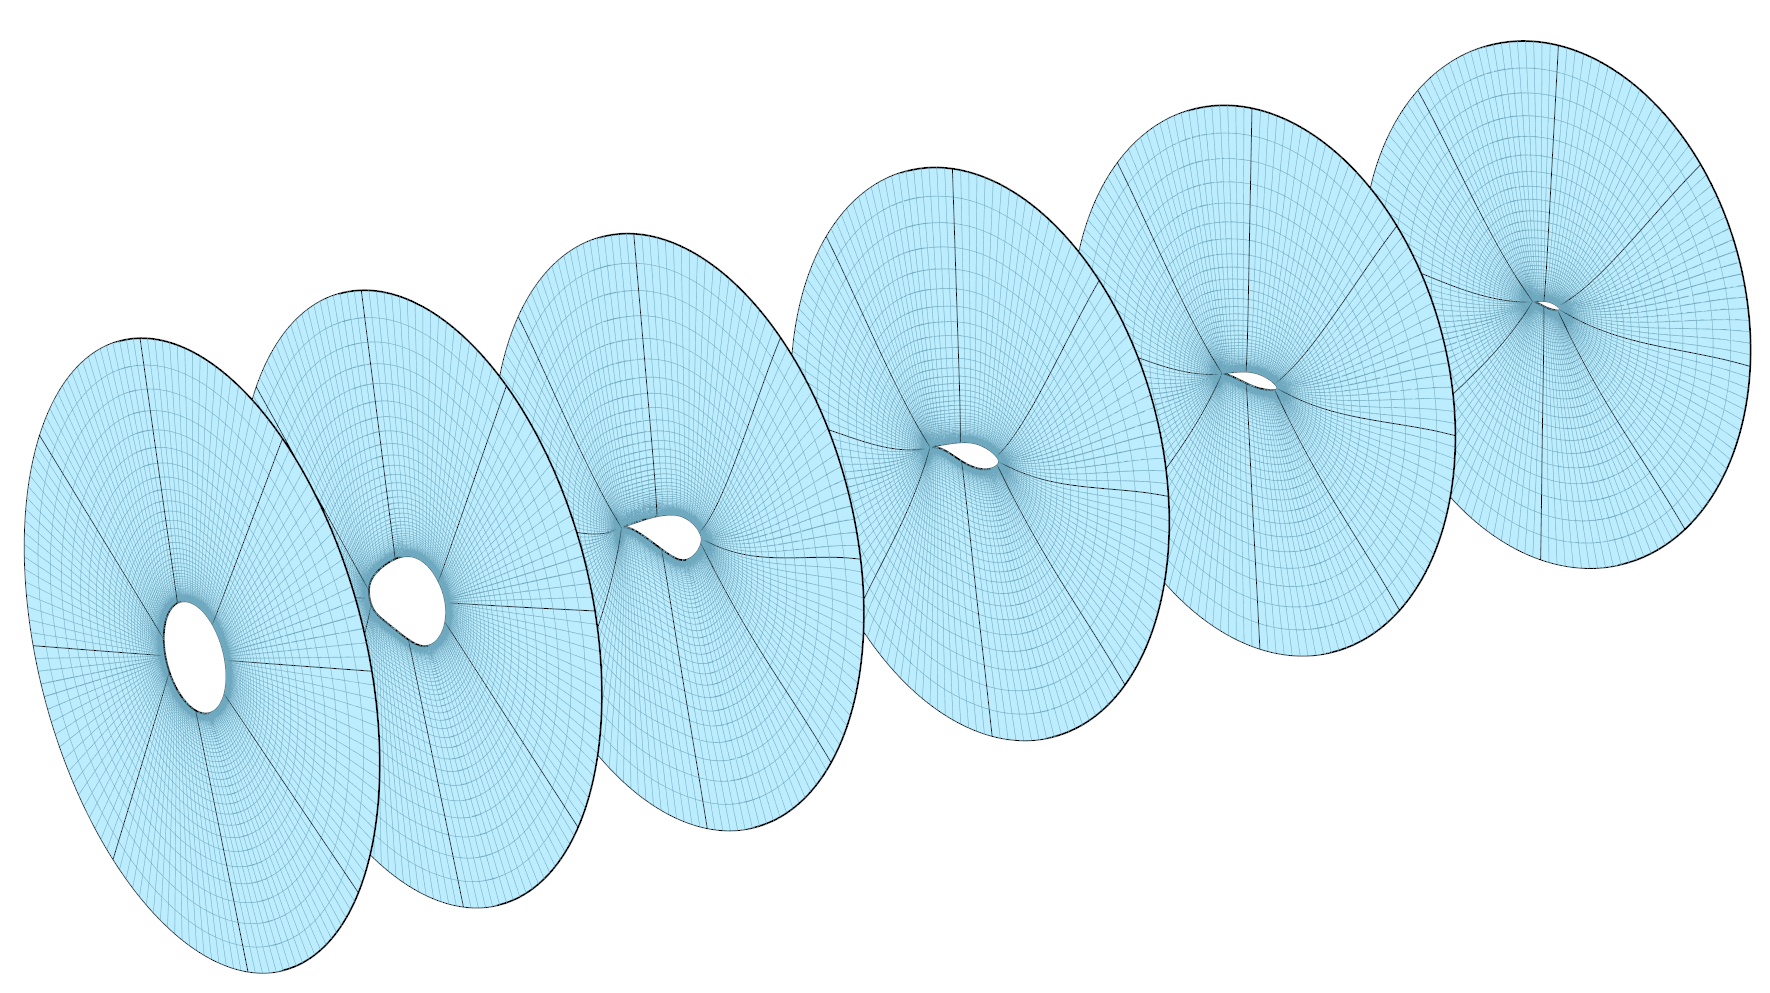
\includegraphics[width=0.32\textwidth]{Figures/crossecs2}}
      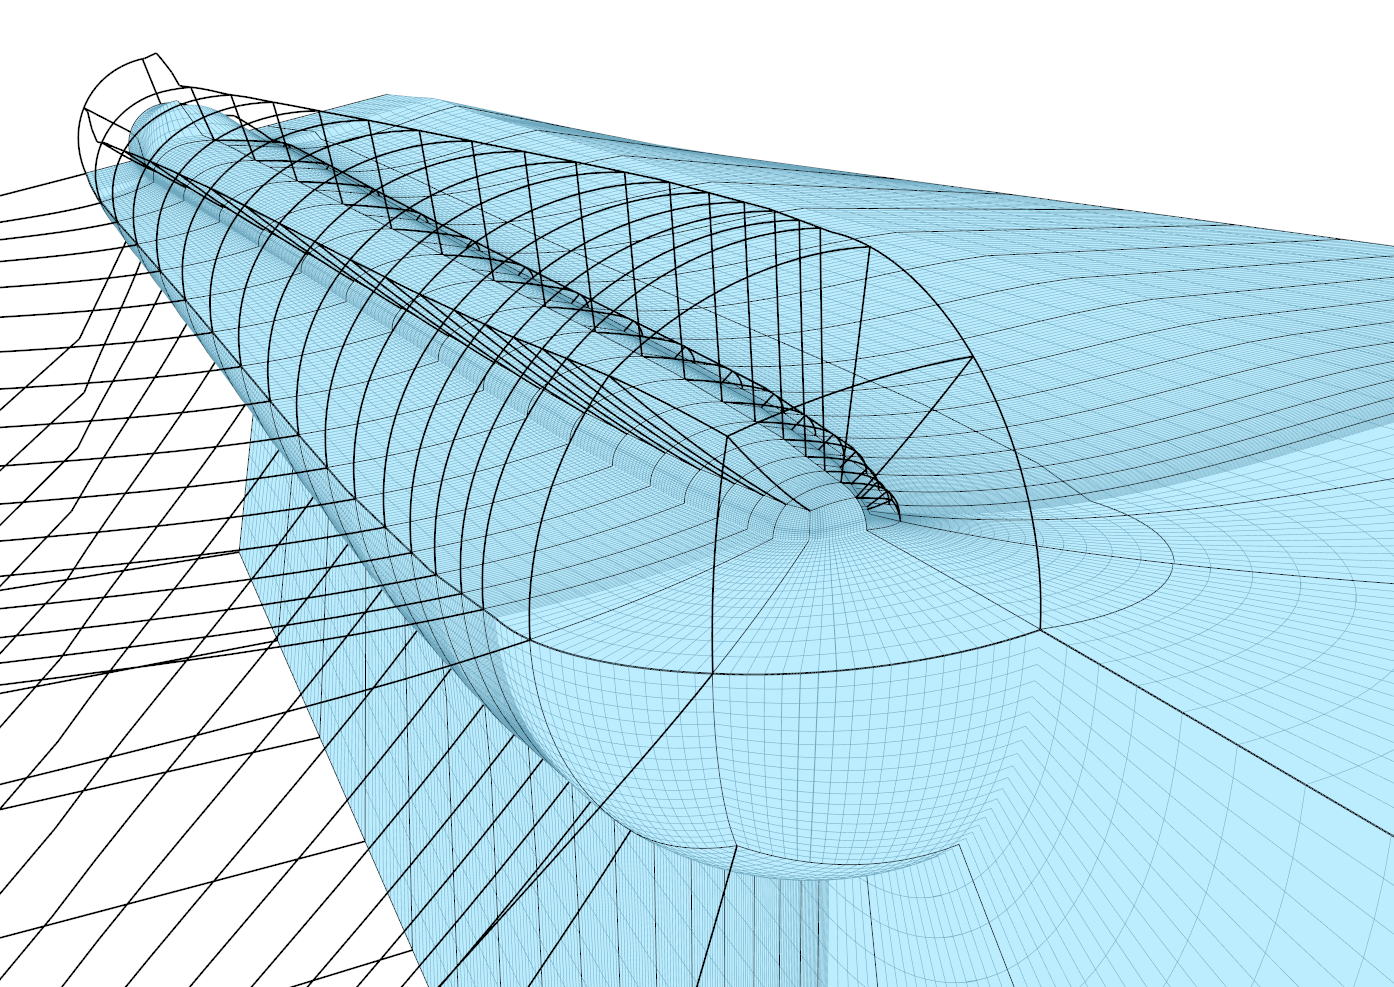
\includegraphics[width=0.32\textwidth]{Figures/block-2} \\
      \normalsize{
        Fig 5: Line-to-surface construction of ``flower mesh'' around a wingtip.
      }
    \end{center}
  \end{figure}
\end{tcolorbox}

\begin{tcolorbox}[colback=white,colframe=sintefblue,title=Integration with Nutils]
  The package is distributed through the Python Package Index (PyPI) and can be installed by typing
  \begin{tcolorbox}[colback=sinteflightgrey]
  \begin{Verbatim}[fontsize=\small]
import splipy.surface_factory as sf
from nutils import *
surf = sf.disc(r=3, center=(2,2))
domain = mesh.rectilinear(surf.knots())
ns = Namespace()
ns.cp = splipy_to_nutils(surf)
ns.phi = domain.basis('spline', p=2)
ns.x = 'phi_n cp_ni'
A = domain.integrate(ns.eval_ij('phi_i,k phi_j,k'))
u = A.solve() \end{Verbatim}
  \end{tcolorbox}
  \begin{figure}
    \begin{center}
      
\includegraphics[width=0.2\linewidth]{right.png} \\
      See also: the stand on nutils
    \end{center}
  \end{figure}
\end{tcolorbox}

\section{Conclusion}

Write som summary things here.
Maybe even box it all in.

{\small \textbf{Disclaimer:}
Splipy does not contain a graphical user interface.
All figures produced on this poster have been created using 3rd party visualizers.
Splipy is to be considered an API ready to be integrated into other custom applications.
}

\end{multicols}

\end{document}

